\section{Evaluation}
\label{sec:eval}

In this section, we build an action concept lexicon for 3734 English
verbs, evaluate its quality and show the effective of
our lexicon on several applications.
We present the datasets and preprocessing.
Then, we evaluate the accuracy and overlap of the lexicon built.
We further show the parameter tuning
and report the execution times of the AC algorithm.
After that, we evaluate the action concept's ability to
identify different senses of verbs by matching
the action concepts to WordNet synsets.
Finally, we show the effectiveness of this lexicon in
four NLP applications:
argument identification, word sense disambiguation,
action frame generation and term similarity.

\section{Data Collection}
\label{sec:data}

To the best of our knowledge, available large scale 3D Bin Packing order dataset is very rare, especially with real-sized items. For that purpose, we create a dataset on 3D bin packing problem of real-world E-commerce platform. This L3DBPD consists of two parts: the customer order data is collected from Taobao\footnote{\url{https://www.taobao.com/}} E-commerce platform and item size data (with length, width and height) is collected from Cainiao\footnote{\url{https://www.cainiao.com/}} Logistics platform. We randomly sampled 150,000 training data and 150,000 testing data for customer orders with 8, 10 and 12 items, which are named as BIN8, BIN10 and BIN12 respectively. We use one line to demonstrate one customer order.

\begin{table*}[!h]
	\small
	\centering
	\caption{Examples of L3DBPD. }
	\label{dataset table}
	\begin{tabular}{|c| c | c | c | c | c | c | c | c | c |}
		\hline
		Order ID & item1  & item2 & item3 & item4  & item5 & item6 & item7  & item8  &  baseline \\  \hline
		1   & (140,50,180) & (100,70,60)  & (170,150,40) & (130,70,40) & (190,150,20)  & (190,150,20) & (240,200,160) &
		(160,170,50)  & 432600  \\ \hline
	\end{tabular}
\end{table*}


Take Table \ref{dataset table} as an example of BIN8, the first and last columns indicate the order ID of a customer order and the heuristic baseline of this BPP, the contents of the remaining 8 columns respectively shows the length, width and height of each items that belong to this order.
We believe this dataset will contribute to the future research of 3D bin packing problem. \footnote{The data will be published soon after accepted.}

\subsection{Accuracy (P-R) and Overlap (vs. SP)}
\label{sec:accuracy}
We run AC algorithm on Web and Google datasets,
using either MI or TF-IDF as the confidence function to obtain
action concept lexicon for $k=1 \dots 10$, 
and for both subjects and objects of all verbs in
Verb-20. We set the parameter $\tau=0.2$, which will be discussed
in \ref{sec:decision_tau}.
%As an example, \tabref{tab:top5result} shows the
%top 5 object concepts for Verb-20 extracted using MI on Web data.
In this section, we show the accuracy of the action concepts
and the degree of their overlaps for each verb in Verb-20.
Our baseline is the top $k$ concepts learned by
selectional preference (SP)\cite{resnik1996selectional}.
SP computes the selectional association between a semantic class $c$
and a predicate $p$ as:
\begin{equation}
A(p,c)=\frac{Pr(c|p)\log\frac{Pr(c|p)}{Pr(c)}}
{\sum_{c'\in C}{Pr(c'|p)\log\frac{Pr(c'|p)}{Pr(c')}}},
\end{equation}
where $C$ is the collection of semantic classes.
%This score measures the difference between the prior probability
%$p(c)$ and posterior distribution
%$p(c|p)$. A large difference stands for high co-occurrence of $c$ and $v$,
%and hence the class and the verb are strongly coupled.

%Since we mainly focus on evaluating the object concepts extracted by
%our approaches, we abuse using the term \emph{argument}
%to refer to object of the verbs in the following experiments.
%\begin{table}[th]
%\caption{Top 5 Object Concepts Extracted by AC on the Web Data}
%\center
%\small
%% Table generated by Excel2LaTeX from sheet 'Sheet1'
%\begin{tabular}{|l|l|}
%    \hline
%    Verb  & Object Concepts\\
%    \hline \hline
%    bring	&person,issue,item,material,factor\\
%    \hline
%    carry	&weapon,product,name,species,factor\\
%    \hline
%    connect	&device,system,component,area,technology\\
%    \hline
%    cut	&material,part,factor,accessory,issue\\
%    \hline
%    define	&group,event,feature,factor,document\\
%    \hline
%    eat	&food,plant,dish,ingredient,flavor\\
%    \hline
%    help    &person,community,company,organization,group\\
%    \hline
%    hit	&place,feature,artist,application,item\\
%    \hline
%    keep	&information,name,item,area,feature\\
%    \hline
%    operate	&system,facility,service,device,technology\\
%    \hline
%    perform	&task,procedure,service,activity,method\\
%    \hline
%    play    &game,character,player,activity,name\\
%    \hline
%    read	&book,information,newspaper,site,classic\\
%    \hline
%    release	&information,name,product,material,player\\
%    \hline
%    report	&crime,event,infection,species,organization\\
%    \hline
%    select	&item,name,topic,feature,company\\
%    \hline
%    spend	&time,money,fund,occasion,festival\\
%    \hline
%    submit	&information,document,datum,documentation,material\\
%    \hline
%    visit	&site,place,community,attraction,name\\
%    \hline
%    wear	&clothing,item,style,accessory,device\\
%    \hline
%    \end{tabular}%
%\label{tab:top5result}
%\end{table}


\subsubsection{Accuracy}
We use precision, recall and $F_1$ measure to evaluate our
algorithm and the generated lexicon.

\textbf{Precision}:
%We use precision to evaluate the quality of concepts produced by each
%algorithm.
For a given verb, a good concept for an argument type
(subject or object) not only covers as many as arguments in the dataset,
but also contains few entities that are invalid for that verb.
The precision score for each verb is:
\[
Precision = \frac{\sum_{c \in C_k}|E_c|\times Precision(c)}
{\sum_{c \in C_k}{|E_c|}},
\]
\[
Precision(c)=\frac{|\mbox{Entities in~} c
\mbox{~which are correct arguments}|}{|E_c|}.
\]
%where $|E_c|$ is the number of entities in concept $c$ and
%$C_k$ is the set of 10 argument concepts discovered by the algorithms.
%We build a ground truth dataset for Verb-20 by
Annotating all entities for each concept needs a large
amount of human efforts. We use a sample strategy to
estimate $Precision(c)$ for a concept $c$. Specifically,
we sample 10 entities from each of the $k$ argument concepts
for each verb learned by the AC and SP.
%discovered by the algorithm.
%To make more typical entities to be more easily sampled out,
%the sampling is conducted according to the typicality of the entities.
%The resulting annotation set comprises 2000 unique entities.
Each entity is then labeled whether it is a correct argument to the
verb by majority of three human judges.
We compare the our algorithm, i.e., AC(MI) and AC(TF-IDF) to
SP in terms of precision on both Web and Google.
The overall precision of the 20 verbs
is reported in \figref{fig:precision_web} and \figref{fig:precision_ngram}.
%For all the algorithms, we keep the top-k concepts for the argument of
%each verb.
For the Web data, as the number of concepts $k$ grows, the precision generally
decreases in all methods. For the Google data, the precision is relatively
stable across different values of $k$.
%This phenomenon indicates that the smaller scale of
%the data causes smaller disparity of the overall quality for different size of concepts we get.
In both datasets, AC(MI) outperforms AC(TF-IDF) and
SP by significant margins. AC(TF-IDF) gives low precision,
perhaps because the TF-IDF scoring doesn't penalize the incorrect arguments
sufficiently but instead prefers to select more general
concepts to maximize the score (\eqnref{eq:approxf}).
%The greedy solution loses in terms of precision
%comparing to local search and selectional preference because it prefers
%to select general concepts to minimize the number of concepts.
%Simulated annealing is able to jump out of the local optimal and
%find a solution that close to the global optimal.
%The comparison among the three approaches on web sentence dataset
%shows that our local search algorithm is enable to find concepts
%with proper granularity, i.e., covering most correct arguments but
%less incorrect arguments. We also compare the precision of
%applying local search to web sentence data with that to Google
%syntactic N-grams.

\textbf{Recall}: Recall measures the coverage of
correct arguments of a verb by the lexicons.
We create two gold standard datasets to evaluate
the recall of action concepts extracted from the
two datasets, i.e., Web and Google.
We manually label 100 correct arguments for each
verb in Verb-20 from both the Web and Google dataset.
These correct arguments are collected randomly and evaluated
by three human judges. With the ground truth, we check
if those correct arguments are covered by one of the concepts
extracted by each algorithm.
The definition of recall for each verb
is computed as below.
$$
Recall=\frac{\sum_{a \in A_v}{I(a,C)}}{|A_v|},
$$
%where
%$A$ is the set of arguments in the web/Google dataset for the verb;
%function $I(a,C)$ is defined as:
$$
I(a,C)=
\begin{cases}
1 & \mbox{if}~ \exists c \in C\ \mbox{and}\ a\ \mbox{IsA}\ c,\\
0 & \mbox{otherwise.}
\end{cases}
$$

We report the recall of our algorithms %, i.e., AC(MI) and AC(TF-IDF)
as well as SP in \figref{fig:recall_web} and \figref{fig:recall_ngram}.
%Greedy solution achieves a very high recall, because
%it prefers larger concepts. Local search and selectional
%preference performs similar in terms of recall.
On both datasets, AC(MI) and AC(TF-IDF) perform much better than SP.
Using TF-IDF as the confidence function achieves a higher recall, because it
tends to select larger concepts, which may decrease the precision
on the contrary as we have discussed.

\textbf{$F_1$ measure}: We examine the $F_1$ measure to
incorporate the precision and recall for an overall
evaluation of the accuracy of the algorithms.
%$F_1$ is
%define as follows:
%$$
%F_1=\frac{2\cdot Precision \cdot Recall}{Precision + Recall}.
%$$
The $F_1$ measure of all three algorithms on the two datasets are summarized in
\figref{fig:f1_web} and \figref{fig:f1_ngram}.
%Greedy solution is fast and achieves good accuracy
%in the top three concepts, while appears to be less efficient
%when the number of concepts become large.
%Local search outperforms
%selectional preference in all settings.
From the figures, we conclude that AC(MI) and AC(TF-IDF) achieve
higher accuracy than SP on both datasets.
%and AC(MI) performs better than AC(TF-IDF).
Because MI has better capability of suppressing low quality entities
than TF-IDF, it achieves the highest overall accuracy.
Generally, AC achieves much higher and more stable accuracy
on both Web and Google data with different values of $k$ than SP.
This is because we consider the concept diversity of the generated concept
lexicon, while SP just selects the top concepts with the highest
preference scores. As such, SP concepts tend to have higher overlap
with each other as we show next.
\begin{figure*}[th]
\begin{minipage}[t]{0.5\columnwidth}
\centering
\epsfig{file=figure/precision_web.eps,width=\columnwidth}
\caption{Precision - Web}
\label{fig:precision_web}
\end{minipage}
\begin{minipage}[t]{0.5\columnwidth}
\centering
\epsfig{file=figure/recall_web.eps,width=\columnwidth}
\caption{Recall - Web}
\label{fig:recall_web}
\end{minipage}
\begin{minipage}[t]{0.5\columnwidth}
\centering
\epsfig{file=figure/f_web.eps,width=\columnwidth}
\caption{$F_1$ Measure - Web}
\label{fig:f1_web}
\end{minipage}
\begin{minipage}[t]{0.5\columnwidth}
\centering
\epsfig{file=figure/overlap_web.eps,width=\columnwidth}
\caption{Overlap - Web}
\label{fig:overlap_web}
\end{minipage}
\end{figure*}

\begin{figure*}[th]
\begin{minipage}[t]{0.5\columnwidth}
\centering
\epsfig{file=figure/precision_ngram.eps,width=\columnwidth}
\caption{Precision - Google}
\label{fig:precision_ngram}
\end{minipage}
\begin{minipage}[t]{0.5\columnwidth}
\centering
\epsfig{file=figure/recall_ngram.eps,width=\columnwidth}
\caption{Recall - Google}
\label{fig:recall_ngram}
\end{minipage}
\begin{minipage}[t]{0.5\columnwidth}
\centering
\epsfig{file=figure/f_ngram.eps,width=\columnwidth}
\caption{$F_1$ Measure - Google}
\label{fig:f1_ngram}
\end{minipage}
\begin{minipage}[t]{0.5\columnwidth}
\centering
\epsfig{file=figure/overlap_ngram.eps,width=\columnwidth}
\caption{Overlap - Google}
\label{fig:overlap_ngram}
\end{minipage}
\end{figure*}

\subsubsection{Overlap}
The overlap score reflects the concepts diversity of the generated lexicon.
The intuition is that the more overlap the pairwise concepts have,
the lower diversity does the lexicon have.
In this section, we evaluate the average pairwise overlap between
extracted action concepts.
%Ideally the intersection between every two concepts in the result
%should be as small as possible, which means each concept should
%correspond to a distinct meaning.
We compute the average overlap score as:
\[
Overlap_{avg} = \frac{2\times \sum_{c_1,c_2\in C_k}{Overlap(c_1,c_2)}}{k(k-1)},
\]
where $C_k$ is the set of top $k$ argument concepts discovered by
the algorithms; $Overlap(c_1,c_2)$ is computed by \eqnref{eq:overlap}.
The results are shown in  \figref{fig:overlap_web} and
\figref{fig:overlap_ngram}.
%The intuition is that, if there is no overlap between
%every two concepts, each argument will be covered by only one concept,
%then overlap score will be 0 which is the best.
%The more overlap, the more concepts one object being covered,
%so that the overlap score will be high. The overlap score of action concepts extracted by the three algorithms
%as reported in \figref{fig:overlap_web}.
%\KZ{Need to revise the following:
%Most of the verbs do not overlap in greedy solution,
%because when we pick a concept we choose from concepts that do not violate the overlap
%constrain. Overlap of local search is slightly higher than GS, but it still guarantees
%the overlap constrain. In contrast, selectional preference tends to generate general
%concepts which results in a high overlap score.
%}
The concepts generated by AC(MI) overlap much less with each other than
AC(TF-IDF) or SP. Because SP does not consider the diversity of concepts,
the Overlap score is much higher. The SP lexicon thus contains many concepts
possessing the same or very similar meanings.
As AC(TF-IDF) prefers general concepts, the Overlap score is also
higher.

Since AC(MI) generally outperforms AC(TF-IDF) in both accuracy and
overlap, MI is adopted as the confidence function in all subsequent experiments.
As $k=10$ generally produces good $F_1$ score and reasonable overlaps, in the
following experiments, unless otherwise noted, $k=10$.

\subsection{The decision of parameter $\tau$}
\label{sec:decision_tau}
One parameter of AC is the overlap constraint $\tau$.
%we should decide it in order to carry on the next potential applications.
To decide the value of $\tau$, we compute
$F_1$ score for the different settings of $\tau$ (from $0.05$ to $0.5$)
by setting $k=10$ for Verb-20.
\figref{fig:f1_vs_tau} shows the distribution of the maximum $F_1$ score against $\tau$.
Each point stands for a verb in Verb-20.
In the figure, we observe that by setting $\tau$ from $0.1$ to $0.25$, we can obtain an optimal
result for most verbs.
We further calculate the deviation of the $F_1$ score at $\tau=0.2$
from the maximum $F_1$ score for each verb, i.e.,
\[dev(v) = F_1(v)_{max} - F_1(v)_{\tau=0.2},\] 
and plot the distribution of these deviations on all 20 verbs 
in \figref{fig:variance}.
The figure shows that most of verbs achieve maximum $F_1$ score
or are very close to the maximum $F_1$ when setting $\tau=0.2$.
Therefore, for simplicity, we set $\tau=0.2$ for all subsequent experiments.

%\begin{figure}[th]
%\centering
%\epsfig{file=figure/f1_vs_tau.eps,width=.65\columnwidth}
%\vspace*{-2ex}
%\caption{$F1_{max}$ against $\tau$}
%\label{fig:f1_vs_tau}
%\end{figure}
\begin{figure}[th]
\begin{minipage}[t]{0.49\columnwidth}
\centering
\epsfig{file=figure/f1_vs_tau.eps,width=\columnwidth}
\caption{Maximum $F_1$ against $\tau$}
\label{fig:f1_vs_tau}
\end{minipage}
\hfill
\begin{minipage}[t]{0.49\columnwidth}
\centering
\epsfig{file=figure/variance.eps,width=\columnwidth}
\caption{Distribution of deviation from $F_1(v)_{max}$}
\label{fig:variance}
\end{minipage}
\end{figure}

%\begin{table}[th]
%\caption{The deviation between $F_1(\tau=0.2)$ to the maximum $F_1$}
%\center
%\small
%\begin{tabular}{|l|l|l|l|l|}
%\hline
%bring&carry&connect&cut&define\\
%\hline
%0.01 & 0.02 & 0.02 & 0.04 & 0.04\\
%\hline
%eat&help&hit&keep&operate\\
%\hline
%0.05 & 0.00 & 0.03 & 0.00 & 0.00\\
%\hline
%perform&play&read&release&report\\
%\hline
%0.02 & 0.00 & 0.04 & 0.03 & 0.02\\
%\hline
%select&spend&submit&visit&wear\\
%\hline
%0.00 & 0.05 & 0.00 & 0.00 & 0.01\\
%\hline
%\end{tabular}
%\label{tab:f1_deviation}
%\end{table}

\subsection{Execution Times}
\label{sec:efficiency}
We record the running times of our branch-and-bound algorithm
for four configurations on a machine with Intel i7-4770 3.4GHz
CPU and 32GB memory, and report them in \tabref{tab:time}.
We ignore the time for sorting candidate concepts because that
is a preprocessing step whose result can be shared by all verbs.
%\GY{whose result can be reused by the verb for the next times.}
Typically the preprocessing takes just under 1 minute.
The times reported are averaged on 3 independent runs for each verb.
The table shows that our algorithm is
efficient enough to generate the action concept lexicon for most verbs.
The running times on Probase are much longer than those on WordNet,
because the concept space of Probase is much larger than WordNet
(14,262,280 concepts in Probase versus 17,157 synsets in WordNet).
\begin{table}[th]
\centering
\caption{Running Times for four Configuartions}
\begin{tabular}{|l|c|c|} \hline
Datasets \& Taxonomies  & Avg. per Verb (sec) & Total (sec) \\ \hline \hline
Web + Probase &	2.244	& 8380.513 \\ \hline
Google + Probase & 1.132 &	2628.488\\ \hline
Web + WordNet&	0.003 &	12.363\\  \hline
Google + WordNet &	0.002	& 5.611	\\ \hline
\end{tabular}
\label{tab:time}
\end{table}
\vspace{-2mm} 

\subsection{Verb Sense Matching}
\label{sec:synset}
The sense of a verb may be identified by the semantic class of its argument.
For example, the verb ``play'' in ``play sports'' holds different
sense to ``play music'' or ``play someone''.
Our lexicon contains strong relations between
verbs and argument concepts, which may indicate certain senses of
the verbs. Here, we evaluate our lexicon on its ability of identifying
verb senses (synsets) with different action concepts.

Each synset of a verb in WordNet contains a gloss, which is an example
sentence illustrating the use of the verb in a particular sense.
From these glosses, we extract verb-subject and verb-object pairs
to construct two test sets, namely Verb-Subject and Verb-Object, respectively.
When a verb has both subject and object in the gloss,
we put its verb-object relation into the verb-object set.
For each verb $v$ in each test set, we run AC and SP with $k$ equal to the
number of senses of $v$,
which is essentially the number of glosses containing $v$.
Let the set arguments (from glosses) covered by the $k$ concepts ($C_k$)
of our lexicon be $A_{g,v}$.
We define the precision
and recall of the mapping as:
\begin{eqnarray*}
Precision(v) &=& \frac{\mbox{min \# of}\ c\in C_k\ \mbox{covering}\ A_{g,v}}{k},\\
Recall(v) &=& \frac{|A_{g,v}|}{k}.\\
\end{eqnarray*}

The precision indicates how many action concepts are needed to
capture all senses of the verb, while recall measures how many
senses can be covered by the action concepts.
%Then, we perform a maximum matching with the Hungary algorithm
%between the $k$ concepts and the arguments extracted from the $k$ glosses
%to check how many senses of the verb we can match.
We also compute the $F_1$ score for the two algorithms and summarize the results
in \tabref{tab:verbmatch}.
%\begin{table}[th]
%\centering
%%\scriptsize
%\caption{Percentage of Maximum Matching between Action Concepts and Arguments in Glosses}
%\begin{tabular}{|l|l|l|}
%\hline
%Test Set & AC & SP \\
%\hline \hline
%Verb-Subject & {\bf 19.54\%} & 11.97\%\\
%\hline
%Verb-Object & {\bf 27.95\%} & 18.67\%\\
%\hline
%Average & {\bf 27.06\%} & 17.26\%\\
%\hline
%\end{tabular}
%\label{tab:verbmatch}
%\end{table}
\begin{table}[th]
\centering
%\scriptsize
\caption{Performance of Verb Sense Matching}
\begin{tabular}{|l|c|c|c|c|c|c|}
\hline
\multirow{2}{*}{Test Set} & \multicolumn{3}{c|}{AC} & \multicolumn{3}{c|}{SP}\\
\cline{2-7}
& Precision & Recall & $F_1$ & Precision & Recall & $F_1$\\
\hline
Verb-Subject &\bf 0.19 &\bf 0.21 &\bf 0.19 & 0.11 & 0.13 & 0.12\\
\hline
Verb-Object &\bf 0.26 &\bf 0.31 &\bf 0.28 & 0.17 & 0.21 & 0.18\\
\hline
Average &\bf 0.26 &\bf 0.30 &\bf 0.27 & 0.16 & 0.19 & 0.17\\
\hline
\end{tabular}
\label{tab:verbmatch}
\end{table}

AC achieves $0.27$ $F_1$ score, while SP gets $F_1=0.17$.
The reason is that SP selects general
concepts which may have higher overlap against each other,
hence they focus on a few senses but miss out other smaller, less
popular senses.

\subsection{Argument Identification (vs. SRL and ReVerb)}
\iffalse Take another corpus and parse it with dependency parser, have human label the
correctness. We may need to artificially inject errors if there's not enough
incorrect action instances. Now use our lexicon, ReVerb and SRL to verify
the correctness and then compare the correlations with the human labels.

If a sentence contains logically or syntactically incorrect argument, then
the method is supposed to identify that.\fi

In the argument identification task, we use our lexicon to examine
whether an argument is correct to a verb in a sentence. To evaluate
the accuracy of argument identification, we first generate a set of
annotated $<$verb, obj$>$ pairs from sentences extracted from Wikipedia
articles. Since using wrong argument in human writing is rare case in daily life, especially
for the high quality online Encyclopedia, the
negative examples of $<$verb, obj$>$ pairs are dominated by the positive
ones, which makes it difficult to observe the differences in accuracy
among the lexicons. We adopt an exchange based method to generate artificial
wrong examples. First, we sample 1000 sentences that contains the verbs in
Verb-20 from Wikipedia and extract action instances from it. Then, we
randomly exchange the arguments with arguments of any other verb. For
example, we exchange ``clothing'' in ``wear clothing'' with the ``piano''
in ``play pinao'' and get two wrong examples ``wear piano'' and ``play clothing''.
We repeat this exchange process several times. Finally, we manually
label the correct arguments in the 1000 sentences, resulting in a test set
consists of around half wrong examples.

%We generate a new dataset consists of 1000 items within each containing a sentence, (target verb,obj) pair and human label.
%First we produce a new corpus consists of sentences randomly selected from Wikipedia for
%verbs in Verb-20.
%Then we randomly select 50 sentences for each target verb in which the verb's direct object exists.
%All the direct objects are collected and for each sentence,
%an alternate object is sampled from the object set.
%We switch the origin direct object and the newly sampled
%one in the sentence and assure that the alternate is still parsed as the verb's object.
%Finally, the new verb-obj pairs are manually labelled for plausible or not.


We compare our lexicon to ReVerb and SRL as follows:
\begin{description}\setlength{\itemsep}{-\itemsep}
\item[Action] Check if the object is an instance of the top k concepts of the target verb.
\item [ReVerb] Check if the object is contained in the object list of the target verb in ReVerb.
\item [SRL(Semafor\cite{chen2010semafor})] We use SRL tool "Semafor" to label the sentence with frame defined by FrameNet, then we check if the object is contained in a frame of the target verb.
\end{description}

\begin{figure}[th]
\centering
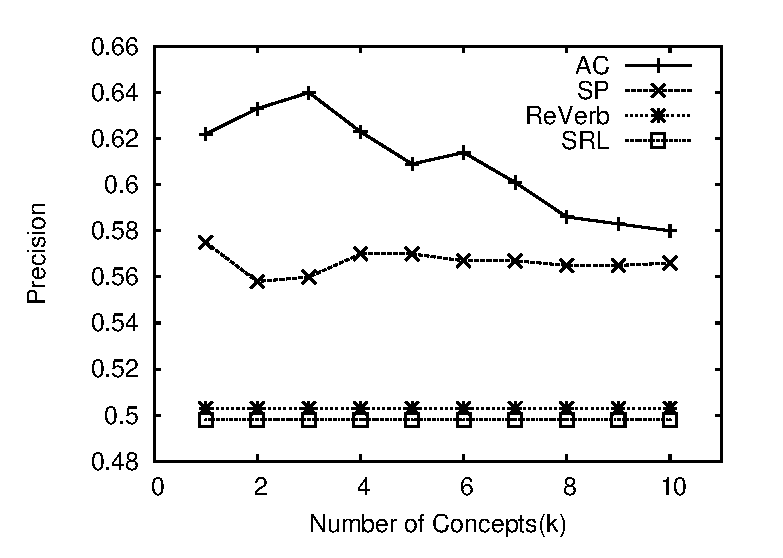
\epsfig{file=figure/argument_identify.eps,width=.65\columnwidth}
\caption{Argument Identification}
\label{fig:argumentidentify}
\end{figure}

We can see from Figure \ref{fig:argumentidentify} that Action's precision is much more better than ReVerb and SRL, and ReVerb is slightly better than SRL. In Action's result, precision are higher with less concepts, indicating high quality concepts are ranked high in our algorithm. Precision becomes stable when number of concepts reaches 7, with minor
deviation.


\subsection{Word Sense Disambiguation}
\label{sec:wsd}
We compare our action concept lexicon with the lexicon extracted
using SP in the lexical sample
word sense disambiguation (WSD) task of
Senseval-3\cite{senseval3}.
Because we focus on using the relation between verbs and
nouns to help WSD,
we extract the training and test cases from Senseval-3
that contain a verb-argument relation
where the verb is in Verb-3734 and the argument is the target noun to be
disambiguated. These relations form our dataset, which consists of
1156 cases for training and 564 cases for testing.

%\KZ{Mention IMS?}
We use the lexicon learned from WordNet in this experiment.
For each target noun to be disambiguated, we extract
the corresponding verb in the context. We then use the
top 10 concepts/synsets of the verb and their
the corresponding scores (i.e., $\tilde{f}(C_k)$ in
\eqnref{eq:approxf} for AC and the selectional
association score for SP) in the lexicon as the only features
to train a linear classifier to classify the sense
for the target noun. The lexicon learned by AC achieves
$F_1 = 0.25$ versus $F_1 = 0.2$ by SP.
This is because SP has higher
overlap in the top 10 concepts/synsets, which dilutes
the difference between features.

\subsection{Action Frame Generation}
%This subsection evaluates our ability to automatically infer fuzzy clusters of verbs.
We apply our action concept lexicon to action frame generation.
We cluster the verbs into fuzzy clusters and assign each fuzzy cluster
an action frame.
%For example, ``buy'' and ``sell'' have the similar usage
%and meaning of ``business deal''.
%In our action concept lexicon, concepts for their objects are almost the same, they are ``product'', ``service'', ``application'' and ``source''. Therefore, regarding our action concepts as a semantic feature, it is able to process verb clustering task.
Since verbs with similar semantics have similar action concepts in our lexicon,
we cluster the verbs by their action concepts.

With concepts extracted from the dataset, we draw a concept histogram for
each verb, which represents the semantic information.
We use the \emph{Vector Space Model} (VSM) to represent the context.
We define a probability distribution score for each dimension
by the IsA relation between the concept and the argument instance as:
$$
Prob(c,v)=\frac{\sum_{e\in E_c\cap A_v}{\frac{freq(e,v)}{|\{c'|c'\in C_k,
e\in E_{c'}\}|}}}{\sum_{c_i\in C_k}{\sum_{e\in E_{c_i}\cap A_v}{\frac{freq(e,v)}{|\{c'|c'\in C_k, e\in E_{c'}\}|}}}},
$$
where $E_c$ is the set of entities covered by concept $c$ in Probase, $A_v$ represents the set of argument instances
for a verb $v$, $freq(e,v)$ is the frequency of the argument $e$ along with verb $v$ in dataset and $C_k$ is the set of concepts for $v$.
In this experiment, the number of concepts we use is $k=10$.

In order to capture the polysemy of verbs, we apply a Fuzzy C-means
clustering method\cite{dunn73:fuzzycmeans} that may assign an item
to more than one cluster. We adopt \emph{cosine similarity}
to compute the pairwise similarity of contexts.
The fuzzy clustering process returns for each verb the coefficient
of being in each cluster, namely $Co(v,c)$.
%In order to find the
%strongest signal of a verb belonging to a cluster,
We design
the following condition to determine if a verb $v_i$
belongs to a cluster $c_j$:
$$
Co(v_i,c_j) \geq \mu_{v_i} + 3 \times \sigma_{v_i},
$$
where $\mu_{v_i}$ and $\sigma_{v_i}$ represents the mean and
standard deviation of the coefficients of the verb $v_i$
being in a cluster.
In the case that a verb has no strong signal of
belonging to a cluster, we make the verb itself a cluster.
\tabref{tab:cluster} shows an example of the clustering results.
\begin{table}[th]
\small
\center
%\scriptsize
\caption{An example of verb clustering results}
\begin{tabular}{|l|l|}
\hline
ID  &   Verb Cluster \\
\hline \hline
1   &   purchase, rent, sell, buy, ship\\
\hline
\multirow{2}{*}{2}
    &   propose, explain, adopt, model, repeat\\
    &   illustrate, describe\\
\hline
\multirow{2}{*}{3}
    &   estimate, subtract, decrease, measure\\
    &   compute, predict\\
\hline
\multirow{2}{*}{4}
    &   complain, perceive, discourage, acknowledge\\
    &   excuse, recall, mind, forbid, favor, wish\\
\hline
\multirow{2}{*}{5}
    &   crumple, unzip, zip, cling, vibrate\\
    &   crimp, magnetize, buckle, flip \\
\hline
\end{tabular}
\label{tab:cluster}
\end{table}

%To evaluate the result of verb clustering, we view it as a series of decisions,
%one for each of the $N(N-1)/2$ pairs of $N$ verbs in the collection.
%We assign two verbs to the same cluster if and only if they
%are similar. A true positive (TP) decision assigns two similar verbs
%to the same cluster, a true negative (TN) decision assigns two dissimilar
%verbs to different clusters. There are two types of errors we can commit.
%A false positive (FP) decision assigns two dissimilar verbs to the same cluster.
%A false negative (FN) decision assigns two similar verbs to different clusters.
%We show it in \tabref{evaluate}.
%\begin{table*}[th]
%\small
%\caption{Explanation about TP, TN, FP and FN}
%\begin{tabular}{|l|l|l|}
%\hline
% & Same cluster & Different clusters\\
%\hline
%Same class & TP & FN\\
%\hline
%Different classes & FP & TN\\
%\hline
%\end{tabular}
%\label{evaluate}
%\end{table*}

%Here we use the metric of Rand Index (RI)\cite{1961008} to evaluate the clustering
%result, which measures the percentage of decisions that are correct.
%$$
%RI=\frac{TP+TN}{TP+FP+TN+FN}
%$$

To evaluate the quality of the action frames,
we adopt a subset of Levin's Verb Classes as golden standard data,
in which 1104 verbs are clustered to 260 classes. In Levin's work\cite{1415692}, she classifies
over 3000 English verbs according to shared meaning and behavior.
%Levin starts with
%the hypothesis that a verb's meaning influences its syntactic behavior and develops
%it into a powerful tool for studying the English verb lexicon.
We use the Rand Index (RI)\cite{1961008} as a metric to evaluate
the clustering result, which measures the percentage of correct
assignment of verbs to clusters.

%For comparison against the fuzzy clustering result, we implement the algorithm with
%our action concepts and SP concepts, the result is shown below.
We compare the fuzzy clustering results using action concepts against the results using
SP concepts.
We note that the fuzzy c-means has one parameter $m$, which is used to determine the level of cluster fuzziness.
To examine how the parameter affects the overall performance of the algorithm,
we conduct the experiment by varying $m$.
\figref{fig:cluster} illustrates the RI of clusters against the value of $m$.
We use the number of clusters $C=260$, which is the same as the number of
Levin's Classes.
As shown in the figure, the performance of verb clustering
using action concepts as features is better than using SP concepts.
\begin{figure}[th]
\centering
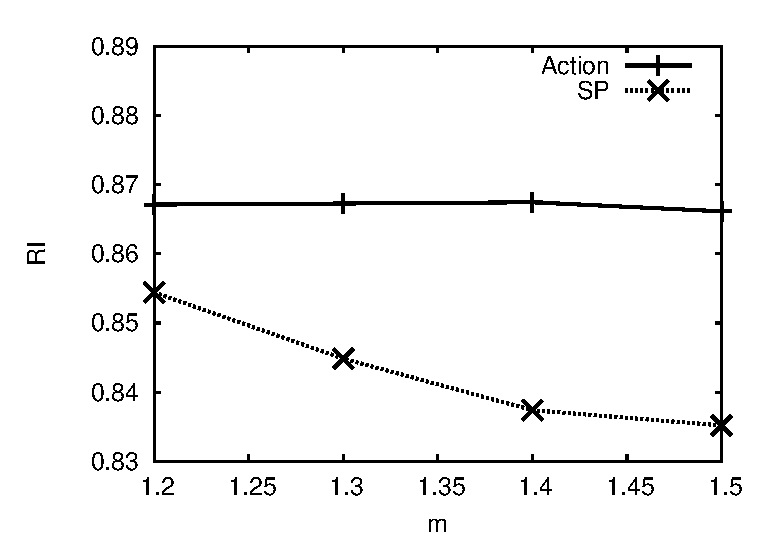
\epsfig{file=figure/cluster.eps,width=.6\columnwidth}
%\vspace*{-5ex}
\caption{RI against fuzzifier $m$}
\label{fig:cluster}
\end{figure}

\subsection{Term Similarity Computation}
% We need the lexicon for large number of verbs... This could be difficult.
Term similarity computation is generally based on a predefined taxonomy.
While computing the similarity of two terms, taxonomy is used to provide
hyponyms and hypernyms information of both terms. Those hyponyms and hypernyms
can be used to represent the terms in set or vector forms, then Jaccard similarity
or cosine similarity can be applied to compute the similarity of the terms.
However, for some ``related'' terms which do not share common hyponyms or
hypernyms, taxonomy may not work well, like ``company'' and ``stock''. We
argue that by complementing our action concept lexicon with taxonomies, we
can obtain a better similarity result. In the example above, ``company'' and
``stock'' can be connected by verb ``release'' or ``sell'', our lexicon can provide
extra knowledge for calculating the similarity of these two terms.

Li\cite{LiWZWW13} introduces a term similarity computation method based on Probase.
In this experiment, we implement Li's method and also define our term similarity
function based on our action concept lexicon. When computing the similarity
of two terms, we combine these two methods and use the higher score produced as
the final similarity score. Similar to Li's method, we apply different similarity
function on terms according to their types(concepts or entities):
\begin{eqnarray*}
sim_{c}(c_1,c_2) &=& \max(\frac{V_o(c_1)\cap V_s(c_2)}{V_o(c_1)\cup V_s(c_2)},\frac{V_s(c_1)\cap V_o(c_2)}{V_s(c_1)\cup V_o(c_2)}) \\
sim_{e}(e_1,e_2) &=& \frac{ \sum_{c_i \in C(e_1)}\sum_{c_j \in C(e_2)} sim_{c}(c_i,c_j) }{|C(e_1)||C(e_2)|} \\
sim_{c\&e}(c,e) &=& \max_{c_i \in C(e)}sim_c(c,c_i)
\end{eqnarray*}
which $V_o(c)$ is the set of verbs taking c as object in action concept lexicon, $V_s(c)$
is the set of verbs taking $c$ as subject. $C(e)$ is the set of concepts for entity $e$ in
Probase.

We test our method(verb based) with Li's method(noun based) on a word similarity label data set
``Word Similarity 353''\cite{LiWZWW13}, using Pearson correlation as the metric. The result is shown below:
\begin{table}[th]
\small
\centering
\begin{tabular}{|c|c|c|}
\hline
Noun based & Verb based & Combined \\
\hline
0.27 & 0.24 & 0.35 \\
\hline
\end{tabular}
\end{table}

We can see that, by combining knowledge provided by Probase taxonomy and our action concept
lexicon, we can get a better similarity result.



